\chapter{Design}

Das folgenden Kapitel beschreibt das User Experience Design für die in Kapitel \ref{sec:analysis} definierten Anforderungen.

\section{Palette}

\section{Authentifizierung}

Das Visual Design für die Authentifizierung (\ref{sec:spec:authentication}) ist in der Abb. \ref{fig:login_form} dargestellt.

\begin{figure}[htp]     % h=here, t=top, b=bottom, p=page
\centering
\includegraphics[width=1.0\textwidth]{images/login_form} 
\caption{Authentifizierung}\label{fig:login_form}
\end{figure}

Der Benutzer gibt hier seine Login Daten ein. Bei positiver Eingabe gelangt er in die Anwendung. Als Standardansicht wird die Photogallerie angezeigt.

\section{Navigations Menü}

Das Navigation innherhalb der Anwendung (Anforderung \ref{sec:spec:menu}) geschieht durch ein von rechts ausklappbares Seitenmenü (Abb. \ref{fig:gallery_large}). Dieses legt sich über den Inhalt im Hauptbereicht der Anwendung. Der Button zum Ausklappen befindet sich in jedem Unterbereich der Andwedung oben rechts (siehe Abb \ref{fig:gallery_normal}). Das Menü nimmt auf kleinen Geräten die gesamte Bildschirmgröße ein.

Zusätzlich bekommt jeder Unterbereich am oberen Bildschirmrand eine spezifische Werkzeugleiste für die Aufgaben des jeweiligen Kontextes. Die spezifischen Werkzeuge haften am rechten oberen Rand.

\begin{figure}[htp]     % h=here, t=top, b=bottom, p=page
\centering
\includegraphics[width=1.0\textwidth]{images/gallery_large} 
\caption{Photo Gallerie Large}\label{fig:gallery_large}
\end{figure}

\section{Photo Gallerie}

Das Design der Gallerie aus Anforerdung \ref{sec:spec:photo_gallery} ist für die Bildschirmgrößen - Large, Normal, Small in den Abb.\ref{fig:gallery_large}, \ref{fig:gallery_normal}, \ref{fig:gallery_small} entsprechend visualisiert.
Generell findet ein Umfluß der Bilder vom mehr auf weniger Spalten statt, bis letztendlich eine einzelne Spalte mit Bildern übrig bleibt.

\begin{figure}[htp]     % h=here, t=top, b=bottom, p=page
\centering
\includegraphics[width=1.0\textwidth]{images/gallery_normal} 
\caption{Photo Gallerie Normal}\label{fig:gallery_normal}
\end{figure}

\begin{figure}[htp]     % h=here, t=top, b=bottom, p=page
\centering
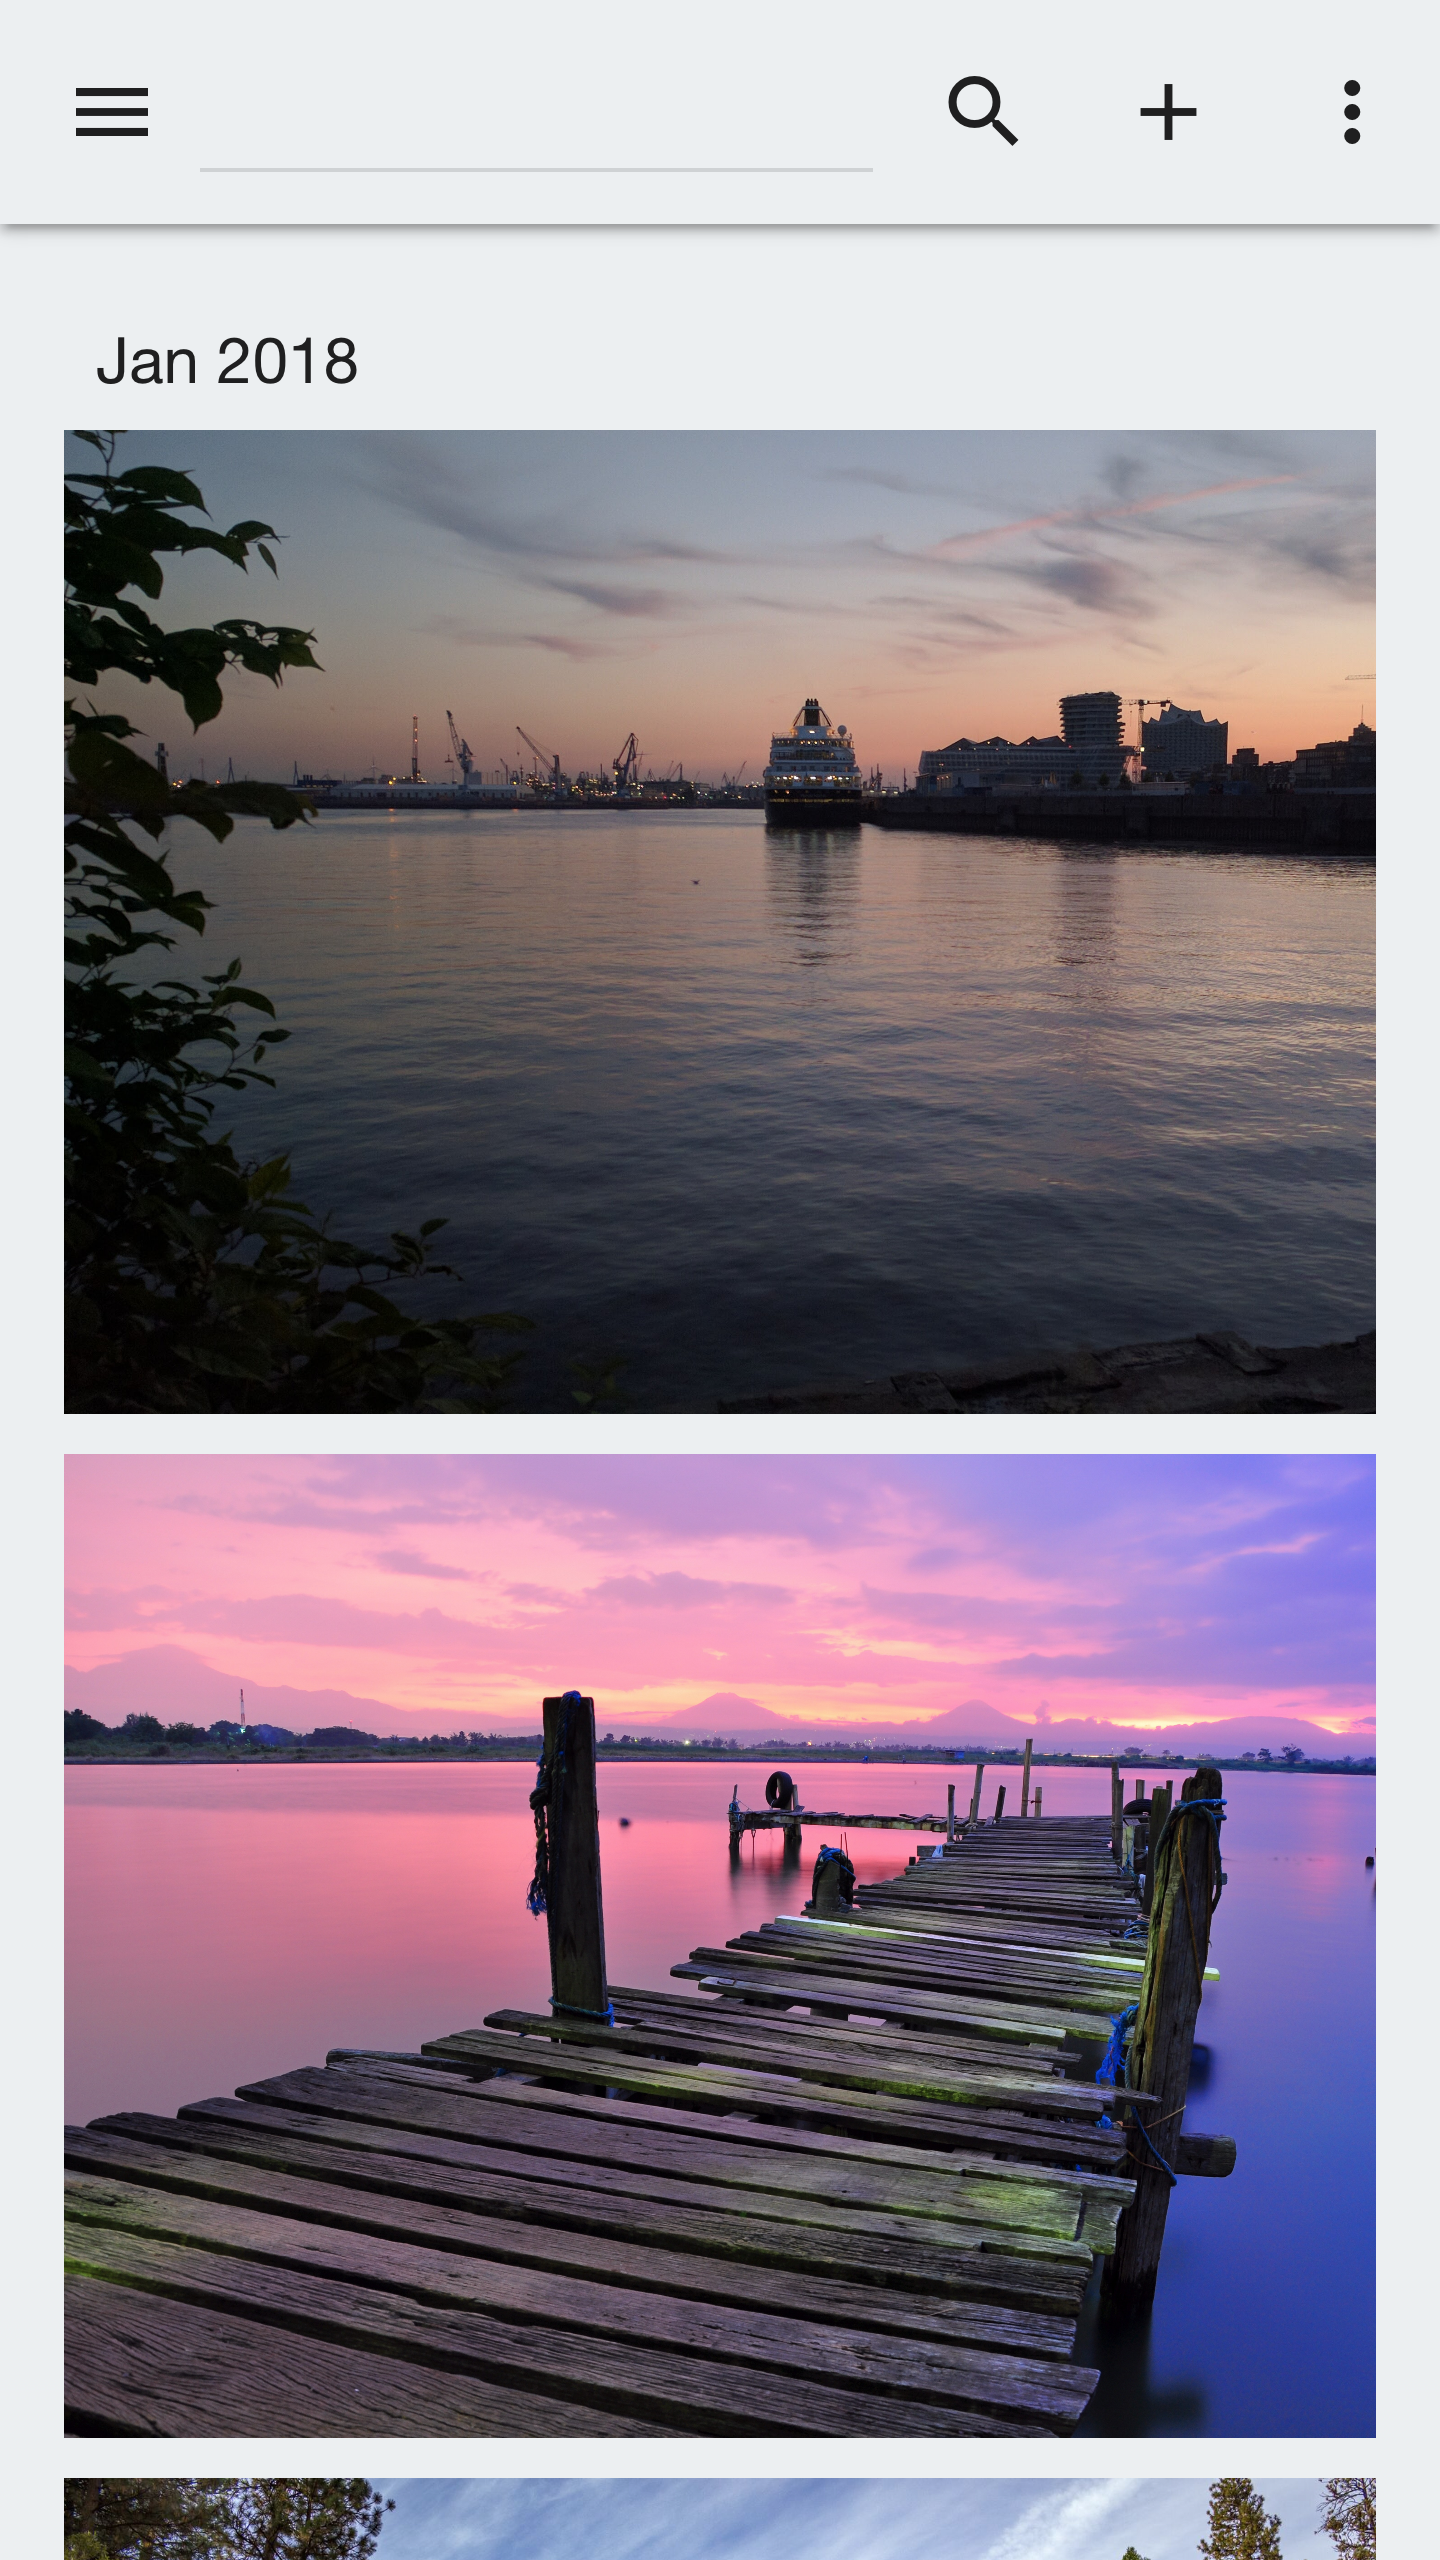
\includegraphics[width=0.5\textwidth]{images/gallery_small} 
\caption{Photo Gallerie Small}\label{fig:gallery_small}
\end{figure}

Die beiden oberen Entwürfe zeigen ebenfalls die Gruppierung der Photos nach dem Erstellungsmonat (Anforderung \ref{sec:spec:photo_groups}) und die ein Suchfeld in der oberen Werkzeugleiste (Anforderung \ref{sec:spec:photo_search}). Die Eingabe eines Suchbegriffs führ instantan eine Suche durch, sobald mehr als 2 Zeichen eigegben werde. Das Ergebnis der Suche ist ebenfalls nach Erstellungsmonat gruppiert.

\section{Paginierung}

Für die Anforderung der Paginierung (\ref{sec:spec:pagination}) bietet die Andwendung dem Benutzer Paginierungs Links für jeweils 2 vorherige und kommende Photobatches ( siehe \ref{fig:pagination}).

\begin{figure}[htp]     % h=here, t=top, b=bottom, p=page
\centering
\includegraphics[width=1.0\textwidth]{images/form_normal} 
\caption{Paginierung}\label{fig:pagination}
\end{figure}

\section{Photo Details}
Die Anforderung der Hauptansicht und Metadaten Betrachtung und Bearbeitung (\ref{sec:spec:photo_details}) ist in dem Visual Design  \ref{fig:form_normal} für die Bildschirmgröße Large abgebildet. Der Benutzer gelangt in die Photo Details Ansicht mit dem Klick auf ein entsprechendes Photo. 

Die Metadaten Ansicht wird mit dem Klick auf das Info Icon von rechts ausgeklappt und ist im Standardzustand nicht sichtbar. Das zentrierte Photo verschiebt sich entsprechend und skaliert im restlichen Bereich.

\begin{figure}[htp]     % h=here, t=top, b=bottom, p=page
\centering
\includegraphics[width=1.0\textwidth]{images/form_normal} 
\caption{Photo Details Normal}\label{fig:form_normal}
\end{figure}

Auf kleineren Geräten nimmt entweder das Photo (Abb. \ref{fig:details_small}) oder das Metadaten Formular den gesamten Platz ein (Abb. \ref{fig:form_small}). 

\begin{figure}[htp]     % h=here, t=top, b=bottom, p=page
\centering
\includegraphics[width=0.5\textwidth]{images/details_small} 
\caption{Photo Details Bild Small}\label{fig:details_small}
\end{figure}

\begin{figure}[htp]     % h=here, t=top, b=bottom, p=page
\centering
\includegraphics[width=0.5\textwidth]{images/form_small} 
\caption{Photo Details Metadaten Small}\label{fig:form_small}
\end{figure}

Die EXIF Kameradaten werden gesondert kategorisiert nach Erstellungsdatum, Kameraeinstellungen und Photodimensionen mit einem entsprechenden Icon pro Kategorie angezeigt.

Die Abbildungen zeigen ebenfalls, dass das betrachtete Photo bei abnehmender Displaygröße proportionell herunterskaliert und immer auf dem Bildschirm zentriert wird (Anforderung \ref{sec:spec:photo_centering}).

Deweiteren sind über dem Photo blaue Pfeile für das Sliden zur nächsten bzw vorheriger Detailansicht eines Photos in den oberen Entwürfen dargestellt. 
(Anforderunge \ref{sec:spec:photo_slider})